\documentclass{contract}

\usepackage{amsmath}
\usepackage{amsfonts}
\usepackage{array} % Required for >{\centering\arraybackslash}
\usepackage{pgfplots}
\pgfplotsset{compat=1.18}

\definecolor{curveblue}{HTML}{0072B2}
\definecolor{curveorange}{HTML}{E69F00}
\definecolor{curvegreen}{HTML}{009E73}
\definecolor{curvered}{HTML}{D55E00}
\definecolor{curvepurple}{HTML}{CC79A7}

\newcommand{\sd}[2]{\ensuremath{\frac{d #1}{d #2}}}
\newcommand{\pd}[2]{\ensuremath{\frac{\partial #1}{\partial #2}}}

\def\f{\hat{f}}
\def\I{\mathcal{I}}
\def\J{\mathcal{J}}

\titletext{Technical Paper}
\subtitletext{The Innovation Game}

%\contractnumber{SDA-2026-001}
\contractdate{\today}
\contracturl{https://tig.foundation/}

\logo{logo_black.png}

\numberwithin{equation}{section}

\begin{document}

\makecontracttitle

\contracttableofcontents

\pagebreak
\section{Optimisable Proof of Work (OPoW)}
\tocdescription{Protocol details for Benchmarker's Proof of Work}

In this section, we outline the mathematical formulas used to compute the rewards and penalties assigned to a Benchmarker $i$ as a result of participation in benchmarking. 
Rewards are assigned to Benchmarker on a \emph{per block} basis, and are computed based on the overall \emph{influence} Benchmarker $i$ exhibits in the reward pool $\mathcal{P}_B$ that is attributed to the Benchmarkers. 
A Benchmarkers influence is composed two main factors: the \emph{challenge factors} and the \emph{deposit factors}.

\subsection{Challenge factors}
\label{sec:challenge-factors}

Let $f_x^i$ be the number of \emph{qualifying} solutions submitted by Benchmarker $i$ for a challenge $x$, such that $x\in X$ where $X$ is the set of all challenges currently available.
For each challenge $x$, there is a set of \emph{challenge tracks} $\tau \in T(x)$, which can vary between challenges. The number of qualifying solutions in a given challenge $f_x^i$ is related to the per track count by a simple summation:
\begin{equation}
    f_x^i = \sum\limits_{\tau \in T(x)}f^i_x(\tau)    
\end{equation}
where $f^i_x(\tau)$ is the number of qualifying solutions for benchmarker $i$ in a challenge $x$ on track $\tau$.
Benchmarkers are incentivized to use `legacy' codes over new submissions which offer only very minor improvements. 
We define the \emph{legacy multiplier} $\mathcal{L}_x(\tau)$ as the a multiplier assigned to each qualifying bundle on each Challenge track, and it is given by  
\begin{equation}
    \mathcal{L}_x(\tau) \in \left[ 1.0 - \frac{S_\mathcal{L}}{2}, 1+ \frac{S_\mathcal{L}}{2} \right]
\end{equation}
where $S_\mathcal{L}$ is the span of the legacy multiplier.
The current configuration sets $S_{\mathcal{L}} = 0.05$, resulting in a range $[0.975,1.025]$.
The legacy multiplier is linearly mapped in this configured range based on the code submission age, in a way that penalizes the newer code submissions and rewards older ones. 

Suppose that there are a total of 3 qualifying bundles $b_1,b_2,b_3$ on a particular challenge track. 
Each bundle is assigned a legacy multiplier a unique value in the range, calculated in regular intervals.
For example, if the age of the algorithm used to produce  the benchmark $b_i$ is $A(b_i)$, and  $A(b_1) > A(b_2) > A(b_3)$, then $b_1$ is assigned the value of 1.025, $b_2$ takes 1.0 and $b_3$ the smallest value of 0.975. 

Different benchmarks will usually share the algorithms used to construct them.
In this case, we assign the legacy multipliers as above, within groups the multipliers are assigned randomly block.
For example, if $A(b_1)> A(b_2) = A(b_3)$, then 0.975 and 1.0 are assigned randomly to $b_2$ and $b_3$ on a per block basis.


% \textcolor{blue}{For example, given that there are a total of 100 qualifying bundles on a challenge track, each bundle is assigned a legacy multiplier within the specified range, in steps of $S_{\mathcal{L}}$/(100-1), according to the age of the code submission which they used for that particular bundle.
% No two bundles have the same legacy multiplier for a given block, and the legacy multiplier can change between blocks.
% If a group of bundles were obtained using the same code submission, the legacy multipliers are assigned randomly in the group for every block.
% }

The average legacy multiplier for Benchmarker $i$ on Challenge $x$ and Challenge track $\tau$ is $\bar{\mathcal{L}}^i_x(\tau)$, and is calculated using a simple mean
\begin{equation}
    \bar{\mathcal{L}}^i_x(\tau) = \frac{1}{f^i_x}\sum_{j=1}^{f^i_x} \mathcal{L}^j_x(\tau).
\end{equation}

For a total of $N_m$, the challenge factor for benchmarker $i$ on challenge $x$ is given by 
\begin{equation}
    \f_x^i = \frac{\sum_{\tau\in T(x)} f_x^i(\tau) \bar{\mathcal{L}}_x(\tau)}{\sum_{i=1}^{N_m}\sum_{\tau\in T(x)}f_x^i(\tau)}.
    \label{eq:challenge-factor-defn}
\end{equation}
The age of a code submission is simply the difference between the current round and the round in which the code was submitted. 
The legacy multiplier incentivizes code innovators to submit codes which offer a relatively significant improvement to the overall state of the art, and newer codes which only offer none or marginal improvements in the quality would not be favorable for Benchmarkers to older,`legacy' codes. 

\subsection{Deposit factors}
\label{sec:deposit-factors}
Alongside the challenge factors, a Benchmarker can earn rewards based on \emph{self-deposits} and \emph{delegations}. 

The self-deposit $d^i_{self}$ is the amount of TIG that a Benchmarker $i$ has deposited.
The delegated amount $d^i_{del}$ is the amount of TIG that have been delegated to the Benchmarker $i$ by other token holders. 
Both of these quantities contribute to the overall reward payout.
The corresponding self-deposit factor $D^i_{self}$ and delegated deposit factors are determined by
\begin{align}
    D^i_{self} &= \min\left\lbrace
    \frac{1.25}{|X|}\sum_{x\in X} \hat{f}^i_x, \frac{d^i_{self}}{\sum_{j=1}^{N_m} d^j_{self}}\right\rbrace\\
    D^i_{del} &= \min\left\lbrace \frac{1.25}{|X|}\sum_{x\in X} \hat{f}^i_x, \frac{d^i_{del}}{\sum_{j=1}^{N_m} d^j_{del}}\right\rbrace
\end{align}
% where $\langle\f_x^i \rangle_{x \in X}$ represents a mean average of the challenge factors across all challenges for the Benchmarker $i$.
Each of these deposits measure Benchmarker $i$'s share of the corresponding total deposits, capped in proportion to the it's average share of qualifying solutions across Challenges.
The variable challenge factor weighting allows us to onboard new challenges smoothly into the protocol.


\subsection{Factor weights}

The challenge factors and deposit factors both contribute to the influence of the benchmarker in the reward pool with an unequal weighting. 
Under the current protocol configurations, the challenge factors are responsible for 75\% of the contribution towards a Benchmarkers influence, while the other 25\% is accounted for by the two deposit factors.

Given a total number of $n$ Challenges, the challenge factor weights $\lbrace w_j^f\rbrace_{j=1}^{n}$ are fixed for all challenges and are determined simply by 
\begin{equation}
    w_j^f = \frac{0.75}{n}
\end{equation}
such that $\sum_{j=1}^{n}w_j^f = 0.75$. The self-deposit $w^{D}_{self}$ and delegated $w^D_{del}$ factor weights are split evenly, with both factors taking an equal weight of $w^D_{self} = w^D_{del} = 0.125$.
The sum of all factors weights is equal to 1. 

\subsection{Influence}
\label{sec:influence}

Let $\mathcal{F}^i$ denote the set of all factors $\lbrace f_1^i,\cdots,f_n^i,D^i_{self},D^i_{del}\rbrace$ for a Benchmarker $i$ and a corresponding weight set $\mathcal{W} = \lbrace w_1^f,\cdots,w_n^f,w^D_{self},w^D_{del}\rbrace$ for each of the entries in $\mathcal{F}^i$.
The size of $\mathcal{F}^i$ is then given by the sum of all challenges and the two deposit factors, i.e $|\mathcal{F}| = n + 2$.  
We now introduce the mean $\mu^i$ and the variance $(\sigma^i)^2$ of $\mathcal{F}^i$, which is given by the standard weighted mean and variance formulae
\begin{align}
       \mu^i &= \frac{\sum_{j=1}^{n+2}w_j f_j}{\sum_{j=1}^{n+2}w_j}\\[2pt]
       (\sigma^i)^2 &= \frac{\sum_{j=1}^{n+2}w_j(f_i - \mu^i)^2 }{\sum_{j=1}^{n+2}w_j}
\end{align}
where $f_j \in \mathcal{F}^i$ and $w_j \in \mathcal{W}$. 
The equality of all factors $f_j$ is called a \emph{parity}. 
Optimisable Proof of Work binds Challenges through a \emph{parity mechanism} that rewards the Benchmarkers that balance their participation across all challenges, self-deposits and tokens delegated from other token holders.
We define the factor imbalance as 
\begin{equation}
    \mathcal{S}^i = \frac{(\sigma^i)^2}{\mu^i(1 - \mu^i)}
\end{equation}
The factor imbalance measures the spread of the factors relative to the largest possible variance at that mean. 
For factors which are similar, $\mathcal{S}_i$ will be small, while a large variation between factors will result in a higher imbalance value $\mathcal{S}_i$. 
A Benchmarker $i$'s \emph{un-normalised influence} is then determined by the mean of the factors, penalised by the imbalance
\begin{equation}
    \mathcal{I}^i = \mu^i \exp(-k\mathcal{S}^i)
\end{equation}
where the parameter $k$ is a fixed `secruity' constant that is set by the protocol.
This parameter $k$ sets the trade between the penalisation of honest specialization and bounding the influence obtainable from a concentrated advantage. 
The current choice for $k$ is set to $k=2$.

\begin{figure}
    \centering
    % plot.tex
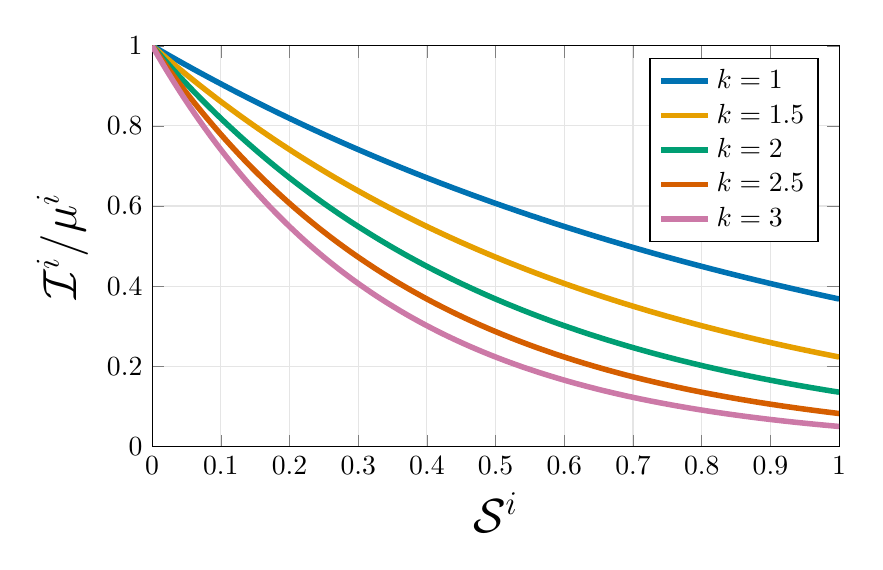
\begin{tikzpicture}
\begin{axis}[
    width=0.85\textwidth,
    height=0.55\textwidth,
    xmin=0, xmax=1,
    ymin=0, ymax=1,
    xlabel={$\mathcal{S}^i$},
    ylabel={$\mathcal{I}^i / \mu^i$},
    xlabel style={font=\fontsize{18}{21}\selectfont},
    ylabel style={font=\fontsize{18}{21}\selectfont},
    legend pos=north east,
    legend cell align=left,
    grid=major,
    major grid style={gray!20},
]
    \addplot[color=curveblue,   line width=2pt, domain=0:1, samples=200] {exp(-1*x)};
    \addlegendentry{$k=1$}

    \addplot[color=curveorange, line width=2pt, domain=0:1, samples=200] {exp(-1.5*x)};
    \addlegendentry{$k=1.5$}

    \addplot[color=curvegreen,  line width=2pt, domain=0:1, samples=200] {exp(-2*x)};
    \addlegendentry{$k=2$}

    \addplot[color=curvered,    line width=2pt, domain=0:1, samples=200] {exp(-2.5*x)};
    \addlegendentry{$k=2.5$}

    \addplot[color=curvepurple, line width=2pt, domain=0:1, samples=200] {exp(-3*x)};
    \addlegendentry{$k=3$}
\end{axis}
\end{tikzpicture}
    \caption{The effect of the security parameter $k$ on the imbalance penalty $\mathcal{I}^i / \mu^i = \exp(-k \mathcal{S}_i)$ for a Benchmarker $i$.}
    \label{fig:imbalance-penalty}
\end{figure}

By construction, the imbalance term $\mathcal{S}^i$ is necessarily bounded in the range $[0,1]$ (see Appendix~\ref{app:relative-variance}). For perfect parity, we have that $S^i = 0$ and no penalty applies to the Benchmarker. 
The maximal penalty for a Benchmarker lies on the other extreme where $S^i = 1$, which corresponds to a penalty of $\exp(-k)$, which corresponds to approximately 86\% reduction of influence. 
The security parameter $k$ is an arbitrary choice, and can be adapted throughout the lifecycle of the protocol in order to ensure fairness, and incentivize the desire for parity (see Fig.~\ref{fig:imbalance-penalty}. 
Increasing the value of $k$ applies stricter penalties on the Benchmarkers influence (see Appendix.~\ref{app:imbalance-penalty}). 


Normalising across all $N_m$ Benchmarkers gives 
\begin{equation}
    \mathcal{J}^i = \frac{\mathcal{I}^i}{\sum_{j=1}^{N_m} \mathcal{I}^j}
\end{equation}
The normalised influence $\mathcal{J}^i$ determines the Benchmarker's expected reward share in the overall Benchmarker reward pool, quantifying the contribution of the Benchmarker across all challenges.
Under a fully decentralized protocol, $\mathcal{J}^i$ also represents the probability that Benchmarker $i$ would produce the next block in the blockchain.   
\subsection{Adoption}

The \emph{adoption} of a code submissions quantifies the overall usage of the code by benchmarkers for a particular challenge.

Benchmarkers are incentivised to use code submissions which maximize their average bundle quality per track. 
As a result, code submissions which on average result in the highest bundle qualities will maximize the profits of both the Benchmarkers (more qualifying bundles scored by the frontier mechanism) and innovators (higher adoption rate which is directly proportional to the innovator rewards in the code submission reward pool). 

The adoption $A_k$ of a code submission $k \in \mathcal{K}$, where $\mathcal{K}$ is the set of all code submissions for some given challenge and block , is given by
\begin{equation}
    A_k = \sum_{i=1}^{N_m}\left( \frac{f^i_k}{\sum_{k'\in\mathcal{K}}f^i_{k'}}\right)\mathcal{J}^i
\end{equation}
where similarily to Sec.~\ref{sec:challenge-factors} we have defined $f^i_k$ as the number of qualifying bundles that a Benchmarker $i$ produced with Code submission $k$. 

As Advance submissions offer a significant improvement to the current state of the art, subsequent code submissions which attempt to improve upon the novel idea introduced by the advance should not be eclipsed by minor improvements. 
The adoption of an Advance submission $m$ is the sum of all of the adoptions of the Code submissions which reference $m$.
Let $K_m$ be the subset $K_m\subset\mathcal{K}$ of code submissions which reference the advance submission $m$.
The adoption $A^m$ of advance $m$ is determined by 
\begin{equation}
    A^m = \sum_{k\in K_m} A_k
\end{equation}
Code submissions reference the Advance submissions Unique Algorithm Identifier (UAI).
There is no automatic penalty applied to Code submissions which improve upon the novelty of the advance submission without referencing it. 
The innovator behind the advance submission is incentivized to report such algorithms to TIG by an unfair loss of tokens through a reduced adoption. 
Reported code submissions are checked internally and banned.

\section{Rewards}
\tocdescription{Reward schemes payable to the players of TIG}

Rewards are payable to players based on the current TIG token  emission schedule, shown in Table.~\ref{tab:emission-schedule}.

\begin{table}[h]
    \centering
    \begin{tabular}{|c|>{\centering\arraybackslash}p{1.6cm}|>{\centering\arraybackslash}p{2cm}|>{\centering\arraybackslash}p{2cm}|c|c|}
    \hline
        Tranche & Rounds & Emissions per block & Emissions per round & Start date & End date \\
        \hline\hline
        1 & 1 - 26 (26) & 100 TIG & 1,008,000 TIG & 24 Nov 2023 & 1 June 2024 \\
        \hline 
        2 & 27 - 78 (52) & 50 TIG & 504,000 TIG & 1 June 2024 & 15 Aug 2025*\\
        \hline
        3 & 79 - 182 (104) & 25 TIG & 252,000 TIG & 15 Aug 2025* & 13 Aug 2027* \\
        \hline
        4 & 183 - 390 (208) & 12.5 & 126,000 TIG & 13 Aug 2027* & 8 Aug 2031* \\
        \hline 
        5 & 391 - 806 (416) & 6.25 & 63,000 TIG & 8 Aug 2031* & 29 July 2039*\\
        \hline
        \end{tabular}
        \begin{flushleft}
        \small\emph{* Approximates}
        \end{flushleft}
    \caption{TIG Token emission schedule.}
    \label{tab:emission-schedule}
\end{table}

Not all of the tokens which are emitted per block are distributed amongst the players, the remaining portion of tokens are temporarily stored within the \emph{TIG vault}. 
The proportion of TIG tokens payable to the players is directy affected by the number of active Challenges in the protocol.
Throughout the lifetime of the protocol, the network is still growing - as new challenges are added the proportion of tokens rewarded to players will increase to an asymptotic value. 

Concretely, we define a scaling function $\Gamma:\mathbb{N} \rightarrow [1,1.02]$ that determines the proportion of emissions to be distributed (with the rest sent to the vault) is based on the current number of active Challenges $n$ such that 
\begin{equation}
    \Gamma(n) = 1.0258(1 - 0.8730e^{-0.0354n})
\end{equation}
As the network approaches a total of 100 active Challenges, $\Gamma(n) \rightarrow 1$ and the rewards payable to the players will coincide with the original token emission schedule.
As the network grows past 100 active challenges, $\Gamma(n)$ will grow asymptotically towards a value of 1.02, and the TIG tokens which were previously stored in the vault are released at a rate of around $2\%$ of the current block token emission rate. 

\subsection{Reward scheme}

\renewcommand*{\thefootnote}{\fnsymbol{footnote}}

Under the current scheme, player reward distribution is performance based and distributed in the following way:
\begin{itemize}
    \item \textbf{Benchmarkers - 50\%}: Distributed amongst Benchmarkers and delegators pro-rata based on each Benchmarker's influence (see Secs.~\ref{sec:benchmarker-rewards} and~\ref{sec:delegator-rewards})
    \item \textbf{Innovators (Advances) - 20\%}: Advance submissions will earn 20\% of the block rewards, which are split evenly across challenges, before being distributed to Innovators, pro-rata with each of the Advance's submission\footnote{In certain cases, rewards may be ``orphaned'', where code/advance submissions may not meet the adoption threshold; or a Challenge may not have an owner. These rewards are redirected into a ``bootstrap'' address in the TIG Treasury, specifically ringfenced to incentivize algorithmic breakthroughs}.
    \item \textbf{Innovators (Code) - 10\%}: These rewards are split evenly across Challenges, before being distributed to Innovators, pro-rata with each of their Code's adoption\footnotemark[1].
    \item \textbf{Challenge Owners (Base) - 10\%}: These rewards are split evenly across all Challenges\footnotemark[1].
    \item \textbf{Challenge Owners (Performance) - 10\%}: There is a secondary reward for Challenge Owners distributed pro-rate with the number of active Advance submissions that have recently been submitted to the Challenge\footnotemark[1]. 
\end{itemize}

The protocol offers a substantially higher reward payout to Challenge Owners and Innovators for advance submissions to incentivize the submission of algorithms that offer signficant improvements to the current state-of-the-art.
Such innovations are of typically substantial commercial value and are strongly encouraged through the reward scheme. 

\subsection{Benchmarker rewards}
\label{sec:benchmarker-rewards}
Benchmarkers receive awards from the Benchmarkers reward pool $\mathcal{P}_B$, such that 
\begin{equation}
    \mathcal{P}_B = R_{block} \cdot r_B
\end{equation}
where $R_{block}$ is the total reward for the block and $r_B$ is the percentage of the block rewards which are shared among all of the Benchmarkers. 
Currently, $r_B$ is set to 0.5, which assigns 50\% of the block rewards to the Benchmarkers. 

A Benchmarker $i$ then receives a reward $R_B^i$ based on the total Benchmarker reward pool and their individual influence by
\begin{equation}
    R_B^i = \mathcal{P}_B \cdot \mathcal{J}^i
\end{equation}

\subsection{Delegator rewards}
\label{sec:delegator-rewards}
Benchmarkers receive awards based on the amount of benchmarking they do, as well as delegated deposits from other token holders.

Delegators are rewarded for their delegations to Benchmarkers by receiving a small share of the Benchmarkers rewards to which they delegated to.

For a Benchmarker $i$, a delegator $d \in \mathcal{D}$ where $\mathcal{D}$ is the set of all delegators receives a reward $R^i_d$ based on
\begin{equation}
    R_d^i = R^i_B\cdot d_s \cdot \frac{d^i_{d}}{\sum_{d'\in\mathcal{D}} d^i_{d'}}
    \label{eq:delegator-rewards}
\end{equation}
where $d_s$ represents the portion of rewards that a Benchmarker $i$ shares to its delegators (set between 0 and 0.25) and $d^i_d$ represents the amount of TIG tokens which are delegated to a benchmarker $i$ by $d$.
By default, the delegator share $d_s$ is set to be 0.15 (15\%) and can be changed on an individual basis by the Benchmarker.
The reward calculation is simply the fraction of the Benchmarker rewards that are shared with the delegators multiplied by the delegator $d$'s contribution to the delegated amount.
The summation in the last term of Eqn.~\ref{eq:delegator-rewards} is nothing more than the delegated amount $d^i_{self}$ in Sec.~\ref{sec:deposit-factors}.

The total reward a delegator $d$ receives from delegating to Benchmarkers is then calculated as the sum
\begin{equation}
    R_d = \sum_{i=1}^{N_m} R^i_d
\end{equation}

\subsection{Code rewards}
\label{sec:code-rewards}

The Code reward pool $\mathcal{P}_C$ constitutes 10\% of the total reward, which is then split equally across all challenges.

Code rewards are calculated based on two different \emph{states}:
\begin{itemize}
    \item Active state: A code submission will become active 4 rounds after it has been submitted.
    \item Merged state: A code submission is merged into the \texttt{main} repository branch if it accumulates enough merge points in a singular round (see Sec.???) 
\end{itemize}

For an active code submission $k\in\mathcal{K}$, the code submission reward $R_k$ is determined based on the overall adoption:

\begin{equation}
    R_k = 
    \begin{cases}
    \frac{\mathcal{P}_C}{n}A_k &  A_k \geq 0.25\\
    0 & A_k < 0.25
    \end{cases}
\end{equation}
where $A_k$ is the adoption and $n$ is the total number of active challenges. 
Code submissions which are in the active state will only be eligible for block rewards if their respective adoption is above $25\%$.
For  algorithms which are in the merged state the adoption threshold is dropped, and the code reward is 
\begin{equation}
    R_k = \frac{\mathcal{P}_C}{n} A_k
\end{equation}
Algorithms which are in the active state but do not exceed the adoption threshold will have their rewards redirected into the TIG bootstrap fund. The total reward that ends up in the TIG bootstrap is simply calculated by 
$$
\frac{\mathcal{P}_C}{n} - \sum_{k\in \mathcal{K}}R_k
$$

\subsection{Advance rewards}
The advance reward pool $\mathcal{P}_A$ constitutes a total of 20\% of the block reward, which is then split evenly across all challenges.
Reward calculations are calculated in much the same way as for the code submissions, with two key differences:
\begin{itemize}
    \item For an advance submission $m$ which is in the active state, the adoption threshold is 50\%. 
    \item Advance submissions rewards are calculated based on all of the code submissions which reference $m$.
\end{itemize}
If $K_m\subset \mathcal{K}$ is the set of all code submissions which reference $m$, the advance reward $R^m$ is given by
\begin{equation}
    R_m = \frac{\mathcal{P}_C}{n}A^m = \frac{\mathcal{P}_C}{n}\sum_{k\in K_m}A_k
\end{equation}
If $K_m = \emptyset$, then the advance submission will not receive any awards.
As in Sec.~\ref{sec:code-rewards}, un-captured rewards are redirected into the TIG Boostrap fund. For a set $\mathcal{M}$ of all advance submissions (for a given challenge and block), the total amount of TIG that ends up in the TIG bootstrap fund is
$$
    \frac{\mathcal{P}_C}{n} - \sum_{m\in M}R_m
$$

\subsection{Challange Owner Rewards}

Challenge owners play an integral part in the lifetime of challenges, by steering the direction and difficulty of Challenges to stay competitive with the state-of-the-art algorithms and ensuring alignment with practical application.

Rewards to challenge owners are payable from a pool $\mathcal{P}_{O_w}$:
\begin{itemize}
    \item A static challenge owner reward pool: Block rewards is assigned as a fixed reward to all Challenge owners.
    \item A dynamic challenge owner reward pool:  A portion of the the block rewards are also set aside as a performance-based reward for challenge owners which are distributed pro-rata based on the number of Recent Advances. 
    If there are no Recent Advances, this reward is evenly distributed to all Challenge Owners. 
\end{itemize}

Recent Advances are defined as advance submissions which have passed the Advance Rewards vote in the past 15 rounds. 
The reward $R_{O_w}$ a challenge owner $O_w$ receives is the sum of their static rewards $R^{stat}_{O_w}$ and dynamic rewards $R^{dyn}_{O_w}$ such that 
\begin{equation}
    R_{O_w} = R^{stat}_{O_w} + R^{dyn}_{O_w} 
\end{equation}
The static reward is computed simply as
\begin{equation}
    R^{stat}_{O_w} = \frac{\mathcal{P}_{O_w}}{n}r_{stat}
\end{equation}
where $r_{stat}$ is a parameter $r_{stat}\in[0,1]$ set to regulate the proportion of the Challenge owner reward pool to assign as a static reward. 
Let $n^i_{adv}$ be the number of recent advances made by challenge owner $i$.
If $\sum_j n^j_{adv} \neq 0$, then the dynamic reward is given by 
\begin{equation}
    R^{dyn}_{O_w} = \frac{n^i_{adv}}{\sum_{j}n^j_{adv}} \mathcal{P}_{O_w}(1-r_{stat})
\end{equation}
If there are no Recent Advances, the dynamic reward for each Challenge owner $i$ is then 
\begin{equation}
    R^{dyn}_{O_w} = \frac{\mathcal{P}_{O_w}}{n}(1-r_{stat})
\end{equation}

\bibliographystyle{plain}
\bibliography{references}

\pagebreak

\appendix
\section{Imbalance penalty}


\subsection{Relative variance}
\label{app:relative-variance}

Given a set of factors $f_i\in[0,1]$ with corresponding weights $w_i \geq 0$ such that $\sum_i w_i = 1$, the weighted mean and variance are determined by
\begin{align}
    \mu &= \sum w_i f_i\\
    \sigma^2 &= \sum w_i (f_i - \mu)^2
\end{align}
In Sec.~\ref{sec:influence}, we defined the imbalance $S$ as the spread of factors 
\begin{equation}
    S = \frac{\sigma^2}{\mu(1 - \mu)}
\end{equation}
In this subsection we will motivate the use of the equation above, often referred to as the bounded variance, to measure the spread of factors.

Suppose that instead, we use the relative variance $S_{CV}$ to define the spread, such that  
\begin{equation}
    S_{CV} = \frac{CV^2}{n - 1}
\end{equation}
where $CV = \sigma/\mu$ is the coefficient of variation with $n-1$ degrees of freedom. 
The relationship between $S$ and the relative variance is given by 
\begin{equation}
    S = S_{CV}\frac{(n-1)\mu}{1 - \mu}
\end{equation}
The difference between the two equations becomes immediately clear when we consider a concrete example.
Consider a set of 4 equally weighted factors, if we compute $S_{CV}$ and $S$ we find that 
\begin{table}[h]
    \centering
    \begin{tabular}{c|cc}
         Factors & $S_{CV}$ & $S$  \\
         \hline
         (0.04,0,0,0) & 1 & 0.0303 \\
         (0,40,0,0,0) & 1 & 0.3333 \\
         (1.00,0.0.0) & 1 & 1
    \end{tabular}
    \label{tab:imbalance-factor-weighting}
\end{table}
Relative variance fails to capture the imbalance of the factors relative to the mean.
Across all three sets, the factors would suffer a maximum penalty under relative variance, even though the parity is much better for the first set compared to the last.
As a result, the calculation of $S$ makes it much easier for smaller participants who might have a smaller share of influence to be involved, as the penalty is balanced with respect to participation. 
Smaller participants suffer smaller consequences for specialisation while larger players are expected to diversify. 
The reason behind this is simple: a smaller participant may not have the sufficient compute to diversify across many challenges. 
Additionally, a small participant will not be able to manipulate the network share through specialisation and as a result does not carry a material risk of market manipulation. 

Both $S_{CV}$ and $S$ lie within the $[0,1]$ under equal weighting. The bounded-variance measure $S$ retains this bound even under unequal weights resulting from the fact that $\sigma^2 \leq \mu(1-\mu)$ is a tight bound~\cite{bhatia2000better}.  


\subsection{Imbalance penalty}
\label{app:imbalance-penalty}
The imbalance penalty is an important mechanic to ensure fairness, and to prevent the domination of a singular Benchmarker in one challenge.
The key consideration that we address here is the choice of the security parameter $k$, which dictates the severity of the imbalance $S^i$ for a Benchmarker $i$. 

Let's suppose that for a given block, we want to directly capture the effect of shifting the value of $k$ on a Benchmarker's influence.
Let $Z(k) = \sum_{j}\mathcal{I}^j$ be the normalisation factor of a Benchmarker $i$'s influence, such that $\mathcal{J}^i = \mathcal{I}^i/Z(k)$ and suppose that $Z(k), \mu^i > 0$.
Taking logarithms, we find that 
\begin{equation}
    \log\mathcal{J}^i = \log\mu^i - kS^i - \log Z(k)
\end{equation}
and then differentiating with respect to parameter $k$ gives
\begin{equation}
    \frac{d\log\mathcal{J}^i}{d k} = - \frac{Z'(k)}{Z(k)} - S^i
\end{equation}
where $Z'(k)$ represents a derivative with respect to $k$.
In fact, we can show that 
\begin{equation}
    Z'(k) = \frac{d}{dk}\left(\sum_j \mu^i e^{-kS^j}\right) = - \sum_j (\mu^j e^{-kS^j})S^j = - \sum_j \mathcal{I}^j S^j = -Z(k) \sum_j \mathcal{J}^j S^j
\end{equation}
We define the influence-weighted average imbalance $\bar{S}_{\mathcal{J}} = \sum_j \mathcal{J}^j S^j$ since $\mathcal{J}^i$ represent the normalized influence weights which sum to 1. 
Substituting, the relative effect of the Benchmarker $i$'s influence due to $k$ is given by an elegant equation
\begin{equation}
    \frac{d\log\mathcal{J}^i}{dk} = \bar{S}_{\mathcal{J}} - S^i
    \label{eq:influence-rate-k}
\end{equation}
From the result above, it is clear how a Benchmarker's influence is sensitive to a change in the value of $k$. For a Benchmarker with a high parity (and therefore a small $S^i$) will have $S^i \leq \bar{S}_{\mathcal{J}}$, and as a result an increase in $k$ should positively affect the Benchmarker's influence, proportional to the deviation from the mean. 
In the opposite direction: a Benchmarker that does not balance their factors well will be negatively affected by an increase in the value of $k$.
If a Benchmarker $i$ has an imbalance penalty $S^i \approx \bar{S}_{\mathcal{J}}$, an instanteneous change in $k$ will not affect the Benchmarker's influence in any significant way. 
It is interesting to note that the imbalance penalty only remains effective as long as the distribution of the $S^i$ values has a sufficiently large variance.
Ideally for the protocol, the distribution of the imbalance $S^i$ should be such that for each Benchmarker $i$, we minimize Eqn.~\ref{eq:influence-rate-k} and therefore minimize the impact of an imbalance penalty.
However this on its own is an insufficient condition to ensure parity.
If there are 4 Benchmarkers and 4 Challenges, and each Benchmarker focused on 1 challenge, $\bar{S}_{\mathcal{J}} = S^i$ for all $i$ and the imbalance penalty is ineffective, and there is no competition within the challenge to drive innovation.  

It should be noted that in Eqn.~\ref{eq:influence-rate-k}, the change in $\mathcal{J}^i$ is only a sensitivity guideline, and it does not imply that for a larger deviation in $k$ the same Benchmarker will continue to either gain or lose influence. 
The influence-weighted average imbalance $\bar{S}_{\mathcal{J}}$ will vary with $k$, and more importantly the equation does not take into account how the influence of one Benchmarker $i$ is affected by a change of factors by another Benchmarker $j$. 
In general, the instantaneous influence shift due to a change in the parameter $k$ is given by 
\begin{equation}
    \mathcal{J}^i(k + \Delta k) = \frac{\mathcal{J}^i(k) e^{-\Delta k S^i}}{\sum_j \mathcal{J}^j(k)e^{-\Delta k S_j}}
\end{equation}

\subsection{Imbalance penalty and market domination}

In an idealised TIG model, the amount of compute which is expended by the Benchmarkers results in an equal share of Challenge factors spread across the challenges for each Challenge.
The security parameter $k$ sets a precedent on how much a Benchmark is penalised by being out of parity.
If the value of $k$ is small, a Benchmarker $i$ may no longer be incentivized to return to parity, on the grounds that forcing compute into a particular challenge will be more profitable than balancing compute across different challenges. 
Without a sufficient driving factor behind penalisation, there is no incentive for a Benchmarker to interact with a particular challenge if the compute will not lead to a substantial increase in reward.  

For example, consider a Benchmarker $i$ who does not have access to a GPU. 
For a sufficiently large $k$, the Benchmarker would incur a large penalty based on not being able to interact with the GPU-based challenges. 
It therefore may be more profitable for the Benchmarker to invest or rent a GPU machine to partake in the GPU-challenges and therefore earn much higher rewards.

There is another motivation behind having a sufficiently large value of $k$.
Suppose that $k$ is very small; a Benchmarker $i$ may intentionally force themselves out of parity in order to gain rewards from another source.
For example, if Benchmarker $i$ decides to submit an algorithm $k$ which may or may not offer a substantial increase to the average bundle quality, they could in theory attempt to funnel all of their compute into this one challenge, and thus earn the adoption rewards from Benchmarking their own algorithms.

The question remains, whether there is some incentive in order to cap the value of $k$ at some larger value. 
If the penalty is large enough, a large Benchmarker could drive an excessive fraction of the total cost into a specific challenge.
Even though a Benchmarker is penalised more heavily through a deviation from parity, they can also push the other Benchmarkers out of parity by pushing more compute into one challenge.
The outcome of this, is that it can become more favourable for a large Benchmarker to drive a higher compute disparity.
In this section, we will show that the turning point at which\textbf{c} a change in one of the challenge factors is no longer detrimental or beneficial, depending on the increment. 

\subsubsection{Benchmarker's influence gradient}

The derivative of the normalised Benchmarker $i$'s influence $\mathcal{J}^i$ with respect to the change in factor $f^j_x$ is given by
\begin{equation}
    \sd{\mathcal{J}^i}{f^j_x} = \sum_{a,b,q,y,z} \pd{\mathcal{J}^i}{\mathcal{I}^a} \pd{\mathcal{I}^a}{\hat{f}_z^b} \pd{\hat{f}_z^b}{f^q_y} \sd{f^q_y}{f^j_x}
\end{equation}
subject to the condition that Benchmarker $j$'s total cost $C^j = \sum_z g^j_z f^j_z$ is held constant, where $g^j_z$ is the unit cost for factor $f^j_z$. 
We now suppose that for Benchmarker $j$, we adjust the value of $f$'s in such a way that the their total cost remains the same. 
This in practise is done by removing compute from one Challenge and inserting it into another. 
Therefore the total rate of change with respect to factor $f_x$ is given by 
\begin{equation}
    0 = \sd{}{f_x}\sum_z g_z f_z = \sum_z g_z \sd{f_z}{f_x} = g_x + \sum_{z\neq x} g_z \sd{f_z}{f_x},
    \label{eq:appendix/cost-derivative}
\end{equation}
where we have dropped the $j$ notation for the Benchmarker. 
Consider now that the Benchmarker increments $c_x = g_x f_x$ by incrementing $f_x$, and that the corresponding changes in $c_{z\neq x}$ are proportional. 
Then it follows that 
\begin{equation}
    \sd{c_z}{c_x} = \sd{(g_z f_z)}{(g_x f_x)} = -q c_z, \quad z \neq x
\end{equation}
where $q$ is a constant of proportionality to be determined. 
From the above, we find that
\begin{equation}
    g_z \sd{f_z}{f_x} = -q g_x g_z f_z,
\end{equation}
and substituting into Eqn.~\ref{eq:appendix/cost-derivative} gives the value of $q$:
\begin{equation}
    q = \frac{1}{\sum_{z\neq x} g_z f_z}.
\end{equation}
Therefore, we find that the derivative is determined by
\begin{equation}
    \sd{f_z}{f_x} = - \frac{g_x f_z}{\sum_{v \neq x} g_v f_v}, \quad z \neq x
\end{equation}
For a general Challenge $y$, the change of one factor with respect to another is given by 
\begin{align}
    \sd{f_y}{f_x} &= \pd{f_y}{f_x} + \sum_{v \neq x} \pd{f_y}{f_v} \sd{f_v}{f_x} \\
    &= \delta_{xy} + \sum_{v\neq x} \delta_{yv} \sd{f_v}{f_x} \\ 
    &= \delta_{xy} + \sum_z \bar{\delta}_{xv}\delta_{yv}\pd{f_z}{f_x}
\end{align}
where $\delta_{xy}$ is the Kronecker delta function, and $\bar{\delta}_{xy} = 1 - \delta_{xy}$. 
Simplifying, we can show that 
\begin{equation}
    \label{eq:appendix/deriv_fy_fx}
    \sd{f_y}{f_x} = \delta_{xy} - \bar{\delta}_{xy} \frac{g_x f_y}{\sum_{v \neq x} g_v f_v}.
\end{equation}
We can now begin with computing the change in influence of Benchmarker $i$. Firstly, we split the derivative using one chain rule definition, which gives
\begin{equation}
    \sd{\mathcal{J}^i}{f_x^j} = \sum_{q,y} \pd{\mathcal{J}^i}{f_y^q} \sd{f_y^q}{f_x^j} = \sum_{q,y} \pd{\mathcal{J}i}{f_y^q}\left(\delta_{qj} \sd{f_y^j}{f_x^j}\right)
\end{equation}
Directly subsituting Eqn.~\ref{eq:appendix/deriv_fy_fx} into the equation above and applying the Kronecker delta we can obtain
\begin{equation}
\sd{\mathcal{J}^i}{f_x^j} = \sum_y \pd{\mathcal{J}^i}{f_y^j}\left(\delta_{xy} - \bar{\delta}_{xy} \frac{g^j_x f^j_y}{\sum_{v\neq x} g^j_v f^j_v}\right)
\end{equation}
The remaining partial derivative can be further expanded by a second use of the chain rule in terms of the normalised challenge factors $\hat{f}_x^j$, such that 
\begin{equation}
    \sd{\mathcal{J}^i}{f_x^j} = \sum_{a,y} \pd{\mathcal{J}^i}{\hat{f}^a_y}\pd{\hat{f}^a_y}{f^j_y} \left(\delta_{xy} - \bar{\delta}_{xy} \frac{g^j_x f^j_y}{\sum_{v\neq x} g^j_v f^j_v}\right)
    \label{eq:appendix/influence-deriv-1}
\end{equation}
To progress further we neglect the Legacy multiplier factor, which here we set to 1 for all tracks and challenges, and assume a uniform weighting across all challenge factors. 
As a result, the normalised challenge factors can be written in the simple form 
\begin{equation}
    \hat{f}^i_x = \frac{f^i_x}{\sum_j f^j_x}.
\end{equation}
Now differentiating the above with respect to challenge factor $f^j_x$, we find that 
\begin{equation}
    \pd{\hat{f}^i_x}{f^j_x} = \frac{\delta_{ij}}{\sum_k f^k_x} + f^i_x \pd{}{f^j_x}\left(\frac{1}{\sum_k f^k_x}\right) = \frac{\delta_{ij}}{\sum_k f^k_x} - \frac{f^i_x / \sum_k f^k_x}{\sum_k f^k_x} = \frac{\delta_{ij} - \hat{f}^i_x}{\sum_k f^k_x}.
\end{equation}
Now substituting the result above into Eqn.~\ref{eq:appendix/influence-deriv-1} results in the following:
\begin{equation}
    \sd{\mathcal{J}^i}{f_x^j} = \sum_{a,y} \pd{\mathcal{J}^i}{\hat{f}^a_y} \frac{\delta_{aj} - \hat{f}^a_y}{\sum_k f^k_y} \left(\delta_{xy} - \bar{\delta}_{xy} \frac{g^j_x f^j_y}{\sum_{v\neq x} g^j_v f^j_v}\right)
\end{equation}
We now make a number of subtle manipulations.
Firstly, multiply the equation above by $\sum_k f^k_x$, to obtain
\begin{equation}
    \sd{\mathcal{J}^i}{f_x^j} = \sum_{a,y} \pd{\mathcal{J}^i}{\hat{f}^a_y} \frac{\delta_{aj} - \hat{f}^a_y}{\sum_k f^k_x} \left(\delta_{xy} - \bar{\delta}_{xy} \frac{g^j_x f^j_y}{\sum_{v\neq x} g^j_v f^j_v}\right) \frac{\sum_k f^k_x}{\sum_k f^k_y}. 
    \label{eq:appendix/influence-deriv-2}
\end{equation}
From the definitions of the normalised challenge factors, we can show that 
\begin{equation}
    \frac{\sum_k f^k_x}{\sum_k f^k_y} = \frac{f^j_x/\hat{f}^j_x}{f^j_y/\hat{f}^j_y} = \frac{\hat{f}^j_y}{\hat{f}^j_x} \frac{f^j_x}{f^j_y}
\end{equation}
Substituting the above into Eqn.~\ref{eq:appendix/influence-deriv-2} gives 
\begin{equation}
    \sd{\mathcal{J}^i}{f_x^j} = \sum_{a,y} \pd{\mathcal{J}^i}{\hat{f}^a_y} \frac{\delta_{aj} - \hat{f}^a_y}{\sum_k f^k_x} \left(\delta_{xy} - \bar{\delta}_{xy} \frac{g^j_x f^j_x}{\sum_{v\neq x} g^j_v f^j_v} \frac{\hat{f}^j_y}{\hat{f}^j_x}\right).  
\end{equation}
Note here that multiplying $\sum_k f^k_x / \sum_k f^k_y$ factor by the Kronecker delta simply leads to the cancellation of the factor, as this is a unitary operation under summation. 
Once more applying the chain rule to the partial derivative that is left, we obtain:
\begin{align}
	\nonumber \sd{\J^i}{f^j_x} &= \frac{1}{\sum_k f^k_x} \sum_{a,y} \delta_{ai} \pd{\J^i}{\I^a}\pd{\I^a}{\f^a}(\delta_{aj} - \f^a_y)\left[\delta_{xy} - \bar{\delta}_{xy} \frac{c^j_x}{\sum_{v\neq x}c^j_v} \frac{\f^j_y}{\f^j_x} \right]\\
							   &= \frac{1}{\sum_k f^k_x} \pd{\J^i}{\I^i}\left\lbrace  \sum_{y} \pd{\I^i}{\f^i_y}(\delta_{ij} - \f^i_y)\left[\delta_{xy} - \bar{\delta}_{xy} \frac{c^j_x}{\sum_{v\neq x}c^j_v} \frac{\f^j_y}{\f^j_x}\right] \right\rbrace
\end{align}
We now focus on the summation term over Challenges $y$, and splitting this into the contributions where $y=x$ and $y \neq x$, such that 
\begin{equation}
	\pd{\I^i}{\f^i_x}(\delta_{ij} - \f^i_x) + \sum_{y \neq x} \pd{\I^i}{\f^i_y}(\delta_{ij} - \f^i_y)\left( \delta_{xy} - \bar{\delta}_{xy} \frac{c^j_x}{(n-1)\langle c^j_{y\neq x}\rangle} \frac{\f^j_y}{\f^j_x} \right)
\end{equation}
where we have used the notation $\langle c^j_{y \neq x}\rangle = \frac{1}{n-1} \sum_{y \neq x} c^j_y$ to denote the average cost of obtaining the challenge factors different from Challenge $x$. 
Now suppose that Benchmarker $j$ is near $\f^j$-parity, such that a single factor at Challenge $x$ is moved away from parity, with the rest remaining the same. 
Additionally, we assume that the rate of change of the unnormalised influence $\I^i$ with respect to the challenge factors is the same for all Challenges different from $x$ near $\f^j$-parity.
Therefore we can simplify the sum in the following way:
\begin{equation}
	(\delta_{ij} - \f^i_x)\pd{\I^i}{\f^i_x} - \frac{c^j_x}{(n-1) \langle c^j_{y \neq x}\rangle} \frac{\f^j_{y \neq x}}{\f^j_x} \pd{\I^i}{\f^i_{y \neq x}} \sum_{y \neq x} (\delta_{ij} - \f^i_y)
\end{equation}
Finally, putting it all together and simplifying we arrive at the general derivative result
\begin{equation}
	\sd{\J^i}{f^j_x} = \frac{1}{\sum_k f^k_x} \frac{\f^j_{y \neq x}}{\langle c^j_{y \neq x}\rangle } \pd{\J^i}{\I^i}\left[(\delta_{ij} - \f^i_x) \frac{\langle c^j_{y \neq x} \rangle}{\f^j_{y \neq x}} \pd{\I^i}{\f^i_x} - (\delta_{ij} - \f^i_{y \neq x}) \frac{c^j_x}{\f^j_x} \pd{\I^i}{\f^i_{y \neq x}} \right]
\end{equation}
Under the assumption that here $i = j$, it immediately follows that:
\begin{equation}
	\sd{\J^i}{f^i_x} = \frac{1}{\sum_k f^k_x} \pd{\J^i}{\I^i}\left[(1 - \f^i_x) \pd{\I^i}{\f^i_x} - (1 - \f^i_{y \neq x}) \frac{c^i_x}{\f^i_x} \frac{\f^i_{y \neq x}}{\langle c^i_{y \neq x}\rangle } \pd{\I^i}{\f^i_{y \neq x}} \right]
\end{equation}
We can make a further simplification that
\begin{equation}
	\frac{c^i_x}{\hat{f}^i_x} = g^i_x \sum_k f^ := h^i_x	
\end{equation}
for both $y=x$ and $y\neq x$ cases (with the latter of course, only holding if the unit costs for all of the $y \neq x$ Challenges .
Interestingly, $h^i_x$ is a measure of the total cost that a Benchmarker $i$ would have to expend in order to obtain a Challenge factor of unity for Challenge $x$.
The derivative re-expressed in terms of these quantities is then
\begin{equation}
	\sd{\J^i}{f^i_x} = \frac{1}{\sum_k f^k_x} \pd{\J^i}{\I^i}\left[(1 - \f^i_x) \pd{\I^i}{\f^i_x} - (1 - \f^i_{y \neq x}) \frac{h^i_x}{h^i_{y \neq x}} \pd{\I^i}{\f^i_{y \neq x}} \right]
	\label{eq:appendix/final-influence-derivative}
\end{equation}
The point at which a change in $f^i_x$ switches from having a beneficial to detrimental effect (or vice versa) on the influence is given by the non-trivial stationary point of the derivative $d \mathcal{J}^i/ d f^i_x$.
The trivial stationary point is obtained by computing
\begin{equation}
\pd{\J^i}{\I^j} = \pd{}{\I^j} \left( \frac{\I^i}{\sum_k \I^k} \right) = \pd{\I^i}{\I^j} \frac{1}{\sum_k \I^k} + \I^i \pd{}{\I^j}\left(\frac{1}{\sum_k \I^k}\right) = \frac{\delta_{ij} - \J^i}{\sum_k \I^k}  
\end{equation}
The above holds for $\J^i = 1$ for Benchmarker $i = j$ and $\J^i = 0$ when $i \neq j$.  
To find the non-trivial stationary point, we set to zero the contents of the square brackets, in order to show that 
\begin{equation}
	\frac{h_x}{h_{y \neq x}} = \frac{1 - \f_x}{1 - \f_{y \neq x}} \frac{\partial \I / \partial \f_x}{\partial \I / \partial \f_{y \neq x}}
\end{equation}
where we have dropped the $i$ notation denoting Benchmarker $i$. 
Defining $p_x = h_x / ( 1 - \f_x)$ as the cost of one extra unit of share in challenge $x$, we arrive at showing
\begin{equation}
	\frac{\partial \log \I / \partial \f_x}{p_x} = \frac{\partial \log \I / \partial \f_{y \neq x}}{p_{y \neq x}}
\end{equation}
where in the equation above we replaced the influence $\I$ with it's logarithm.
The equations which are listed above give rise to some interesting results pertaining to the protection of a Benchmarkers ability to dominate the market.

\subsubsection{Market domination with uncapped qualification}

A Benchmarker $i$'s influence will change with respect to their Challenge factors given by Eqn.~\ref{eq:appendix/final-influence-derivative}
\begin{equation}
\sd{\J^i}{\f^i_x} \propto (1 - \f^i_x) \pd{\I^i}{\f^i_x} - \frac{h_x}{h_{y \neq x}} (1 - \f^i_{y \neq x}) \pd{\I}{\f^i_{y \neq x}}
\end{equation}
Simply put, the first term on the right side of the equation above represents the influence gained from the share that one solution buys in Challenge $x$, while the second term represents the loss of influence you give up from the share that the same cost would have bought in challenge $y$.
The term $1 - \f^i_x$ represents the \emph{dilution} of the influence gained as the Benchmarker $i$ begins to dominate a certain challenge $x$.
As the $\f^i_x \rightarrow 1$, this term falls to 0 and influence gained from additional solutions is diluted down.

The dilution alone provides some protection for the Benchmarking market against domination of a single competitor, even without the addition of an imbalance penalty.
Suppose that we switch off the imbalance penalty by setting $k=0$, and assume that the unit costs of all challenges $g^i_x$ is equal.
To put this into a numerical context, let's assume that you initially start with a total of 100 qualifiers in each challenge, and everyone else has a total of 900 in each challenge.
In this situation it is simple to estimate the challenge factor $\f^i_x = 100/(100 + 900) = 0.1$. 
Now suppose the Benchmarker has access to a larger compute, and is able to generate more qualifying solutions. The results of this numerical experimental are listed in Table.~\ref{tab:appendix/uncapped-equal-unit-costs}

\begin{table}[h]
	\centering
	\begin{tabular}{ccccc}
		$f_x$ & $\f_x$ & Gain $(1 - \f_x)$ & Loss $(h_x/h_y)(1 - \f_{y \neq x})$ & Estimated $d \J / d \f_x$ \\ 
		\hline
		100 & 0.10 & 0.90 & 1.0 \cdot 0.9 = 0.90 & 0\\
		300 & 0.25 & 0.75 & 1.2 \cdot 0.9 = 1.08 & -0.33 \\
		900 & 0.50 & 0.50 & 1.8 \cdot 0.9 = 1.62 & -1.12 \\
       8100 & 0.90 & 0.10 & 9.0 \cdot 0.9 = 8.10 & -8.00
	\end{tabular}
	\caption{Change in Benchmarker's influence $i$'s based on no imbalance penalty and fixed unit costs.} 
	\label{tab:appendix/uncapped-equal-unit-costs}
\end{table}
At parity, the derivate is 0, and every qualifier in Challenge $x$ results in a larger loss of influence than gain.
At 90\%, each solution loses around 8 times as much influence as it gains.
It is interesting to consider the situation, what happens if we no longer assume that the unit costs of obtaining a qualifying solution is a fixed costs. 
Suppose that in this situation, a Benchmarker has access to some special optimisation for challenge $x$ only\footnote{An example of this could be that a Benchmarker has access to an ASIC.} which results in the unit costs $g_x$ of Challenge  $x$ being substantially smaller than for the other Challenges.
To what degree 




\end{document}
